% !TEX root = ../main.tex

\section{Proposed Methodology: The SAARTHI Framework}

SAARTHI runs on a hybrid detection engine built to make the most of the scarce
compute cycles available on an in-cab edge node. The architecture divides into
four logical stages, which we call Zones (Fig.~\ref{fig:framework}); within Zone~3, detection
splits further into two parallel tracks, Track~A and Track~B.

\begin{figure*}[t]
\centering
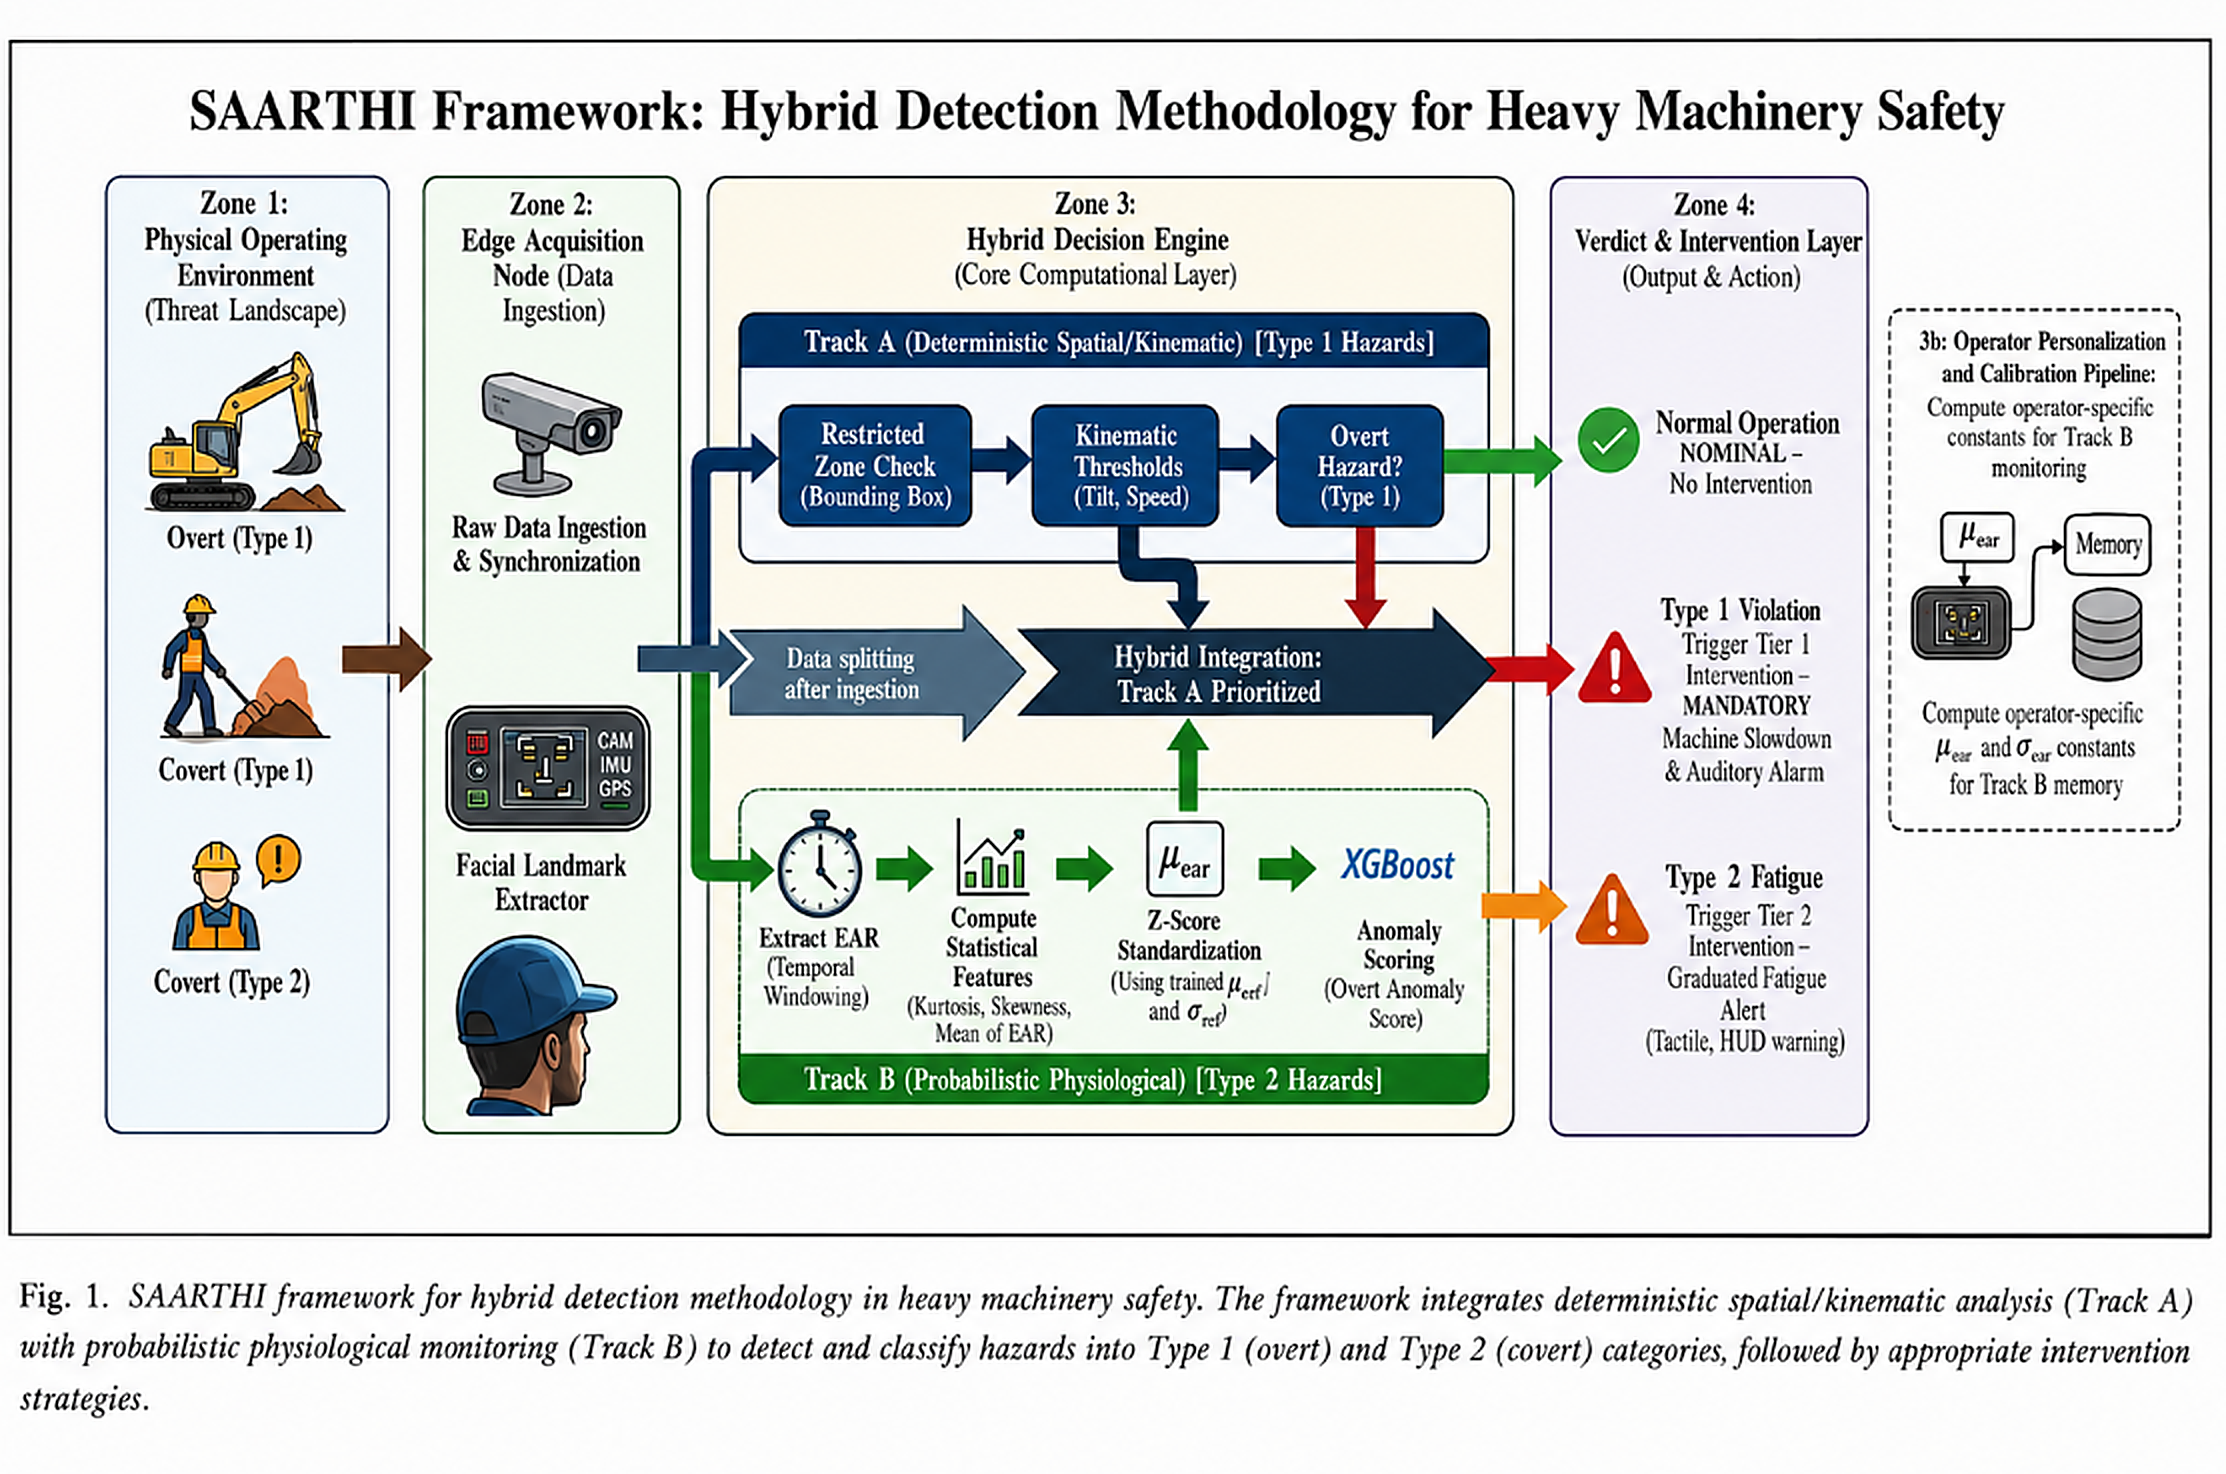
\includegraphics[width=\textwidth]{figures/framework_architecture.png}
\caption{SAARTHI framework for hybrid detection methodology in heavy machinery safety. The framework integrates deterministic spatial/kinematic analysis (Track A) with probabilistic physiological monitoring (Track B) to detect and classify hazards into Type 1 (overt) and Type 2 (covert) categories, followed by appropriate intervention strategies.}
\label{fig:framework}
\end{figure*}

\begin{itemize}
\item \textbf{Zone 1 --- Operating Environment:} The physical threat landscape: the
overt (Type~1) and covert (Type~2) hazards present in and around the heavy
machine.
\item \textbf{Zone 2 --- Edge Acquisition Node:} Raw data ingestion through the
cabin-facing camera and the machine's telemetry interface (e.g.\ the CAN bus).
\item \textbf{Zone 3 --- Hybrid Decision Engine:} The core computational layer, housing
Track~A (deterministic spatial/kinematic rules) and Track~B (XGBoost
physiological anomaly scoring).
\item \textbf{Zone 4 --- Verdict \& Intervention:} The final decision layer, which
outputs the real-time safety status and manages the appropriate Tier-1 or
Tier-2 response.
\end{itemize}

End to end, the pipeline runs in four steps:

\begin{enumerate}
\item \textbf{Ingestion.} Raw video frames and machine telemetry are captured
and synchronized.
\item \textbf{Buffering.} EAR values and machine states accumulate in a size-$w$
circular buffer, forming temporal sliding windows.
\item \textbf{Filtration (Track A).} Visual bounding boxes and kinematic
telemetry (speed, tilt) are checked against deterministic safety constraints
such as restricted-zone violations.
\item \textbf{Verification (Track B).} If Track~A raises no overt hazard, the
statistical physiological features (kurtosis, skewness, rate of change) are
computed and passed to the XGBoost model for covert fatigue scoring.
\end{enumerate}

Splitting the cheap work from the expensive work is the whole point of this
design. By keeping deterministic spatial and kinematic checks (Track~A) separate
from the heavier statistical physiological analysis (Track~B), the system spends
its machine-learning budget only where it is needed. The result is a lower
computational load on the edge device, which keeps thermal throttling at bay and
preserves real-time responsiveness without sacrificing diagnostic precision.

\subsection{Data Acquisition and Adaptive Preprocessing}

The data flow starts in Zone~2, where the cabin-facing camera and the telemetry
bus run continuously. This passive style of monitoring reflects the
non-intrusive philosophy that heavy machinery demands: it sidesteps the
``observer effect,'' since the operator is never asked to check in and is never
pulled away from a delicate task. And rather than processing every frame
indiscriminately, as a standard vision pipeline would, the SAARTHI node
selectively intercepts and synchronizes facial landmarks with CAN bus telemetry.

Because this multi-modal stream arrives fast and the device's SRAM is limited,
the system buffers it in a circular queue. The buffer acts as a shock absorber,
decoupling the irregular rate at which vision primitives are extracted from the
steady clock of the downstream inference engine.

\subsubsection{Circular Buffer Management}

Algorithm~\ref{alg:ingestion} formalizes how the stream is managed. Only valid
frames --- those with an intact face detection and high-confidence landmarks ---
are admitted. To avoid memory fragmentation, a persistent headache on embedded
targets, the buffer allocates its memory statically and overwrites in place,
always favouring the most recent temporal window.

\subsubsection{Feature Engineering and Statistical Standardization}

Once the temporal buffer $B_t$ holds a full window of valid samples, the system
moves into feature engineering. The main challenge here is taming the stochastic
variance in the physiological and kinematic readings, so that the feature vector
$\mathbf{x}$ handed to the classifier is stable enough to trust.

\begin{algorithm}[h]
\caption{Adaptive Rolling Window Data Ingestion}
\label{alg:ingestion}
\KwIn{Raw video stream $S_V$, telemetry stream $S_T$, window size $w$}
\KwOut{Temporal buffer $B_t$}
\Globals{Static ring buffer $R$ of size $w$, head pointer $p$}
\While{System Active}{
    $f_{raw} \gets \mathrm{ReadFrame}(S_V)$\;
    $t_{raw} \gets \mathrm{ReadTelemetry}(S_T)$\;
    \tcp{Stage 1: detection integrity filtering}
    \If{$\mathrm{DetectFace}(f_{raw}) = \textsc{fail}$}{
        \textbf{continue}\tcp*{discard frames lacking a clear face}
    }
    \tcp{Stage 2: extraction}
    $e_{ear} \gets \mathrm{ExtractEAR}(f_{raw})$\;
    $k_{state} \gets \mathrm{ExtractKinematics}(t_{raw})$\;
    \tcp{Stage 3: buffer injection}
    $R[p] \gets \{\, e_{ear},\ k_{state},\ \text{timestamp} \,\}$\;
    $p \gets (p + 1) \bmod w$\;
    \tcp{check window saturation}
    \If{$p = 0$ \textbf{\emph{or}} \textsc{BufferFullFlag}}{
        $B_t \gets \mathrm{Linearize}(R)$\;
        \textbf{Trigger} $\mathrm{FeatureExtraction}(B_t)$\;
    }
}
\end{algorithm}

\subsubsection{Window Size Selection and Stability Criterion}

Choosing the window size $w$ is a metrological trade-off between detection
latency and statistical stability. Empirically, raw detection accuracy peaks at
smaller windows --- but that peak sits squarely in the white-noise-dominated
regime, where frame-to-frame variance (from natural rapid blinks, for example)
runs high. Short windows may look accurate on paper, yet they invite false
positives driven by transient physiological noise.

To put the choice on firmer ground, we ran an Allan deviation analysis over
steady-state operator streams. The noise floor bottomed out at an averaging time
of $\tau_{opt} \approx 30.0$ samples --- the stability plateau, where white noise
is already minimized but random-walk drift (posture shifts and the like) has not
yet taken over. SAARTHI therefore uses $w = 30$, sitting right at $\tau_{opt}$
and trading the marginal sensitivity of smaller windows for operational
stability. At this size the total data-collection time stays under 1.5 seconds,
comfortably inside the $T_{hazard\_onset}$ pre-intervention budget.

\subsubsection{Z-Score Standardization}

XGBoost's decision space is distance-sensitive, and our feature space is
heterogeneous, so the features have to be scaled. Left unscaled, high-magnitude
variables like variance would swamp low-range ones like skewness and tilt the
decision boundary. The system applies Z-score standardization in real time:

\begin{equation}
z_i = \frac{x_i - \mu_{cal}}{\sigma_{cal}}
\label{eq:zscore}
\end{equation}

The constants $\mu_{cal}$ and $\sigma_{cal}$ are fixed during the initial
30-second operator calibration and kept in memory, which spares the device from
recomputing global statistics on every frame. Algorithm~\ref{alg:features}
spells out the full extraction logic.

\begin{algorithm}[h]
\caption{Statistical Feature Extraction}
\label{alg:features}
\KwIn{Temporal buffer $B_t$, calibration stats $(\mu_{cal}, \sigma_{cal})$}
\KwOut{Normalized feature vector $\mathbf{z}$}
\tcp{Compute raw mean (first pass)}
$\mu \gets 0$\;
\For{$i \gets 1$ \KwTo $w$}{
    $\mu \gets \mu + B_t[i].\mathrm{ear}$\;
}
$\mu \gets \mu / w$\;
\tcp{Compute higher-order moments (second pass)}
$\mathit{sum\_sq} \gets 0$;\quad $\mathit{sum\_cu} \gets 0$;\quad $\mathit{sum\_qd} \gets 0$\;
\For{$i \gets 1$ \KwTo $w$}{
    $\mathit{diff} \gets B_t[i].\mathrm{ear} - \mu$\;
    $\mathit{sum\_sq} \gets \mathit{sum\_sq} + \mathit{diff}^2$\;
    $\mathit{sum\_cu} \gets \mathit{sum\_cu} + \mathit{diff}^3$\;
    $\mathit{sum\_qd} \gets \mathit{sum\_qd} + \mathit{diff}^4$\;
}
$\sigma \gets \sqrt{\mathit{sum\_sq} / (w - 1)}$\;
$E_{roc} \gets B_t[w].\mathrm{ear} - B_t[w-5].\mathrm{ear}$\;
$S_k \gets (\mathit{sum\_cu} / w) / \sigma^3$\;
$K_u \gets \big((\mathit{sum\_qd} / w) / \sigma^4\big) - 3$\tcp*{excess kurtosis}
\tcp{Construct and standardize}
$\mathbf{x} \gets [\,\mu,\ \sigma,\ E_{roc},\ S_k,\ K_u\,]$\;
\For{$j \gets 1$ \KwTo $5$}{
    $z[j] \gets (x[j] - \mu_{cal}[j]) / \sigma_{cal}[j]$\;
}
\Return $\mathbf{z}$\;
\end{algorithm}

\subsection{Track A: Deterministic Spatial and Kinematic Verification}

Track~A is a fast, deterministic pre-filter that runs in $O(1)$. Its job is to
catch Type~1 overt hazards the instant they occur --- a pedestrian entering a
restricted zone, an unsafe machine tilt --- with no machine-learning overhead at
all. It does this by testing the current state against a deterministic
constraint set $C_{rules}$, implemented as a lookup over predefined spatial
boundaries and kinematic thresholds.

Bounding-box intersection tests and threshold comparisons cost next to nothing
on any edge processor, so this gate is cheap. Only states that clear Track~A ---
those with no deterministic hazard --- go on to Track~B for the deeper
physiological analysis.

\subsection{Track B: Statistical Physiological Anomaly Scoring (XGBoost)}

Track~B takes on the Type~2 covert hazard, the case where the operator still
looks awake and engaged while the underlying physiological signal quietly drifts
toward fatigue. To catch that drift, the system uses a gradient-boosted ensemble
(XGBoost) trained on the standardized feature vector $\mathbf{z}$.

Most classifiers need labelled ``fatigue'' examples, which are expensive or
simply unavailable for every individual operator. SAARTHI sidesteps that: the
calibration phase learns a personalized envelope of normal operation for each
operator, and any feature vector that strays well outside that envelope is
flagged as a fatigue anomaly.

\subsubsection{The Primal and Dual Formulations}

The ensemble's goal is to carve a decision boundary in the feature space
$\Phi(\mathbf{x})$ that separates the bulk of the training data --- alert
operator states --- from the anomalous region. It does so by learning an
additive ensemble of $T$ weak learners that minimizes a regularized objective:

\begin{equation}
\mathcal{L} = \sum_{i=1}^{n} l(y_i, \hat{y}_i) + \sum_{t=1}^{T} \Omega(f_t)
\end{equation}

where $l$ is the loss, $\hat{y}_i$ the predicted score, and
$\Omega(f_t) = \gamma T + \tfrac{1}{2}\lambda \lVert w \rVert^2$ a penalty on
tree complexity. SAARTHI sets $\lambda = 1.0$ for strict regularization, treating
the outermost 1\% of training samples as candidate edge-case fatigue anomalies.

\subsubsection{The Gradient Boosting Kernel}

A linear boundary cannot capture the tangled, non-linear interplay between
higher-order moments like kurtosis and skewness. To build a surface expressive
enough to resolve them, XGBoost grows trees over the feature space
$\Phi(\mathbf{x})$, in effect approximating a kernel mapping. At inference time
the decision function is:

\begin{equation}
D(\mathbf{z}) = \operatorname{sgn}\!\left( \sum_{t=1}^{T} \eta \cdot f_t(\mathbf{z}) - \rho \right)
\label{eq:decision}
\end{equation}

where $\eta$ is the learning rate and $\rho$ the decision threshold. The
regularizer's $\gamma$ sets the minimum gain a split must earn, which in turn
governs how sharply the boundary curves. Algorithm~\ref{alg:training} outlines
the offline procedure that produces the boosted model shipped to the edge device.

\begin{algorithm}[h]
\caption{Offline Training Procedure}
\label{alg:training}
\KwIn{Training dataset $X_{train}$, params $(\eta, \lambda, \gamma, T)$}
\KwOut{Boosted model $M$, offset $\rho$}
\tcp{Feature matrix computation}
$Z \gets \mathrm{ExtractAndStandardize}(X_{train})$\;
\tcp{Ensemble training}
$M \gets \mathrm{XGBoost.Train}(Z,\ \mathrm{params}(\eta, \lambda, \gamma, T))$\;
\tcp{Extract decision threshold}
$\rho \gets \mathrm{ComputeThreshold}(M, X_{train})$\;
\tcp{Model compression for edge}
$M \gets \mathrm{Quantize}(M, \rho)$\;
\Return $M$\;
\end{algorithm}

When $D(\mathbf{z}) = -1$, the feature vector lies outside the calibrated
operator's learned envelope, and a fatigue alert is raised.

\subsubsection{Hybrid Logic Integration}

At the heart of Zone~3, the final decision logic fuses the deterministic
certainty of Track~A with the probabilistic rigour of Track~B;
Algorithm~\ref{alg:hybrid} lays out the combined flow. Running the lightweight
Track~A check first keeps the heavier XGBoost inference of Track~B on a low duty
cycle.

The final safety verdict is recovered through the ensemble's decision function
in Equation~\eqref{eq:decision}. If $D(\mathbf{z}) = -1$, the signal has fallen
outside the calibrated operator's normal distribution, and a Tier-2 fatigue
intervention fires.

\begin{algorithm}[h]
\caption{Hybrid Execution Flow}
\label{alg:hybrid}
\KwIn{Feature vector $\mathbf{z}$, kinematic state $k_{state}$, rules
$C_{rules}$, model $M$, threshold $\rho$}
\KwOut{Safety verdict $V$, intervention tier}
\tcp{Track A: deterministic gate}
\If{$\mathrm{CheckConstraints}(k_{state}, C_{rules}) = \textsc{violation}$}{
    $V \gets \textsc{hazard\_type\_1}$\;
    \textbf{Trigger} $\mathrm{Tier1Intervention}()$\;
    \Return $V$\;
}
\tcp{Track B: physiological anomaly scoring}
$\mathit{score} \gets \sum_{t=1}^{T} \eta \cdot f_t(\mathbf{z})$\;
\eIf{$\operatorname{sgn}(\mathit{score} - \rho) = -1$}{
    $V \gets \textsc{hazard\_type\_2}$\;
    \textbf{Trigger} $\mathrm{Tier2Intervention}()$\;
}{
    $V \gets \textsc{nominal}$\;
}
\Return $V$\;
\end{algorithm}

\subsection{Tiered Intervention Protocol}

When either track returns a positive verdict, SAARTHI responds with a
structured, tiered protocol rather than a single binary alarm. The graduation
matters in a heavy-machinery setting: a sudden, jarring alert in the middle of a
delicate manoeuvre --- a precise crane lift, say --- could itself cause the
accident it was meant to prevent.

\medskip
\noindent\textbf{Tier 1 --- Deterministic override (Track A).} Fires the instant
a kinematic violation is confirmed --- for example $\theta > \theta_{crit}$ while
$v \neq 0$, or a bounding-box intrusion into a restricted zone. The response is
non-negotiable: a mandatory speed-reduction command goes straight to the CAN bus
and a loud cabin alarm sounds. This tier is independent of operator behaviour or
any machine-learning state.

\medskip
\noindent\textbf{Tier 2 --- Adaptive fatigue alert (Track B).} Fires when
$D(\mathbf{z}) = -1$, signalling a sustained drift outside the operator's normal
envelope. Here the response builds gradually: first a tactile seat-vibration
pulse, then a visual HUD warning if the anomalous state persists beyond
$\delta_t$ consecutive windows. Should the operator not acknowledge within a
preset timeout $T_{ack}$, the system escalates to a Tier-1-equivalent mandatory
slow-down.

\medskip
This restrictive admission-control approach keeps interruptions rare during
normal operation while guaranteeing that genuine hazards always draw an
immediate, deterministic response --- which, in practice, is what earns operator
trust and keeps the system in use.

\subsection{Operator Personalization and Calibration}

Population-level fatigue models share one fundamental weakness: physiology varies
from operator to operator. A naturally narrow-eyed operator's baseline EAR mean
$\mu_{alert}$ can look, statistically, like another operator's fatigued state ---
and the resulting stream of false positives steadily erodes trust in the system.

SAARTHI answers this with a mandatory 30-second calibration at the start of every
shift. The operator is asked to look ahead, relaxed and alert, while the system
ingests $N_{cal}$ frames and computes operator-specific statistics:

\begin{equation}
\mu_{cal} = \frac{1}{N_{cal}} \sum_{i=1}^{N_{cal}} e_i,
\qquad
\sigma_{cal} = \sqrt{\frac{1}{N_{cal}-1} \sum_{i=1}^{N_{cal}} (e_i - \mu_{cal})^2}
\end{equation}

These constants then Z-score-normalize every incoming feature vector
(Equation~\ref{eq:zscore}), anchoring the whole pipeline to the individual's
physiology rather than a generic population mean. Each profile is saved to the
operator profile store, so returning operators skip re-calibration --- though the
profile can still be refreshed over time to track long-term physiological drift.

